%! Author = bedlamzd
%! Date = 28.02.2021

% Preamble
\documentclass[14pt]{extarticle}

%! Author = bedlamzd
%! Date = 16.02.2021

\usepackage{fontspec}
\usepackage{polyglossia}
\defaultfontfeatures{Ligatures=TeX}
\setdefaultlanguage{russian}
\setotherlanguage{english}
\setmainfont{PT Astra Serif}
\newfontfamily{\latinfont}{PT Astra Serif}
\newfontfamily{\cyrillicfont}{PT Astra Serif}
\newfontfamily{\cyrillicfonttt}{FreeMono}

\usepackage{geometry}

\usepackage{amsmath}
\usepackage{amssymb}
\usepackage{amsfonts}
\usepackage{graphicx}
\usepackage{float}
\usepackage{wrapfig}
\usepackage[caption=false]{subfig}

\geometry{right=20mm}
\geometry{left=20mm}
\geometry{top=20mm}
\geometry{bottom=20mm}

\usepackage{indentfirst}
\usepackage[outputdir=out]{minted}

\renewcommand{\theFancyVerbLine}{\ttfamily{\normalsize\oldstylenums{\arabic{FancyVerbLine}}}}

\newminted{python}{autogobble, linenos, fontsize=\small, xleftmargin=2\parindent}
\newmintinline{python}{fontsize=\small}
\newmintedfile{python}{autogobble, linenos, fontsize=\small, xleftmargin=2\parindent,
breakanywhere, breaklines}

\newminted{matlab}{autogobble, linenos, fontsize=\small, xleftmargin=2\parindent}
\newmintinline{matlab}{fontsize=\small}
\newmintedfile{matlab}{autogobble, linenos, fontsize=\small, xleftmargin=2\parindent,
breakanywhere, breaklines}

\renewcommand{\thesubsection}{\arabic{subsection}}

\graphicspath{{../img/}}



% Document
\begin{document}
    \begin{titlepage}
    \begin{center}
        \begin{small}
            \textbf{Министерство науки и высшего образования Российской Федерации}

            \vspace{1em}

            ФЕДЕРАЛЬНОЕ ГОСУДАРСТВЕННОЕ АВТОНОМНОЕ ОБРАЗОВАТЕЛЬНОЕ\\
            УЧРЕЖДЕНИЕ ВЫСШЕГО ОБРАЗОВАНИЯ

            \vspace{1em}

            \textbf{<<НАЦИОНАЛЬНЫЙ ИССЛЕДОВАТЕЛЬСКИЙ УНИВЕРСИТЕТ ИТМО>>}
        \end{small}

        \vspace{13ex}

        Практическая работа №4\\
        <<Планирование движения>>\\
        по дисциплине <<Моделирование и управление робототехническими системами>>
    \end{center}

    \vspace{14em}

    \begin{flushright}
        \noindent
        Выполнил:\\
        студент гр. R41341c\\
        Борисов М. В.

        \vspace{1em}
        Преподаватель:\\
        Каканов М. А.
    \end{flushright}

    \vfill

    \begin{center}
        \large{Санкт-Петербург}\\
        2021 г.\\
    \end{center}
\end{titlepage}


    \section*{Дано}
    Модель двухзвенного робота
    \begin{equation}
        \label{eq:sys}
        M(q)\ddot{q} + C(q, \dot{q})\dot{q} + F\dot{q} +G(q) = u - \tau_\text{dist},
    \end{equation}
    где $q,\ \dot{q},\ \ddot{q}$ --- векторы обобщённых координат, скоростей и ускорений соответственно,
    $u$ --- вектор управляющих воздействий,
    $M(q),\ C(q,\dot{q}),\ F$ --- матрицы инерции, кориолисовых-центробежных сил и вязкого трения соответственно,
    $G(q)$ --- вектор гравитационных сил,
    $\tau_\text{dist}$ --- вектор моментов внешних сил.
    \newline

    Моменты внешних сил
    \begin{equation}
        \label{eq:ext moments}
        \tau_\text{dist}(t) =
        \begin{bmatrix}
            C_{\text{dist},\ 1} + A_{\text{dist},\ 1}\sin(\omega_{\text{dist},\ 1}t + \psi_{\text{dist},\ 1})\\
            C_{\text{dist},\ 2} + A_{\text{dist},\ 2}\sin(\omega_{\text{dist},\ 2}t + \psi_{\text{dist},\ 2})
        \end{bmatrix}
    \end{equation}

    Задающий сигнал
    \begin{equation}
        \label{eq:traject}
        q_{\text{ref}}(t) =
        \begin{bmatrix}
            A_{\text{ref},\ 1}\sin(\omega_{\text{ref},\ 1}t + \psi_{\text{ref},\ 1})\\
            A_{\text{ref},\ 2}\sin(\omega_{\text{ref},\ 2}t + \psi_{\text{ref},\ 2})
        \end{bmatrix}
    \end{equation}

    Цель управления
    \begin{equation}
        \label{eq:goal}
        \lim_{t \rightarrow \inf }\left| q_e(t) \right| = 0,
    \end{equation}
    где $q_e(t) = q(t) - q_\text{ref}(t)$ --- сигнал ошибки.

    \section*{Задание}
    \paragraph*{Задание 1} Синтез робастного регулятора

    \subparagraph{Допущение 1} Робот не подвержен влиянию внешних возмущений, $\tau_\text{dist} = 0$.
    \newline

    \noindent Закон управления
    \begin{equation}
        \label{eq:control no dist}
        u = \bar{u} = \text{sat}_N M_0\left( -\sigma - K\hat{\xi} + u_\text{ff} \right),
    \end{equation}
    где $N$ --- предел насыщения контура управления,
    $K$ --- матрица положительных коэффициентов,
    $u_\text{ff}$ --- управление по прямой связи,
    $M_0$ --- обратимая матрица приближённого момента инерции объекта,
    $\hat{\xi},\ \sigma$ --- состояние расширенного наблюдателя.
    \newline

    Требуется провести численное моделирование замкнутой системы~\eqref{eq:sys},~\eqref{eq:control no dist}
    в режиме слежения за траекторией~\eqref{eq:traject} с обеспечением цели управления~\eqref{eq:goal}.

    \paragraph*{Задание 2} Синтез внутренней модели

    Ослабим Допущение 1 и построим робастный регулятор по выходу с компенсацией внешних возмущений.

    Для этого в структуру регулятора добавляется внутренняя модель, компенсирующая влияние внешнего момента.

    Требуется провести численное моделирование замкнутой системы~\eqref{eq:sys},~\eqref{eq:control no dist}
    с внутренней моделью в режиме слежения за траекторией~\eqref{eq:traject} с обеспечением цели управления~\eqref{eq:goal}
    и компенсации детерменированных внешних возмущений~\eqref{eq:ext moments}.

    \section*{Моделирование}
    \subsection*{Задание 1}
    В пакете MATLAB соберём систему~\eqref{eq:sys} в виде модели Simulink.
    \begin{figure}[H]
        \centering
        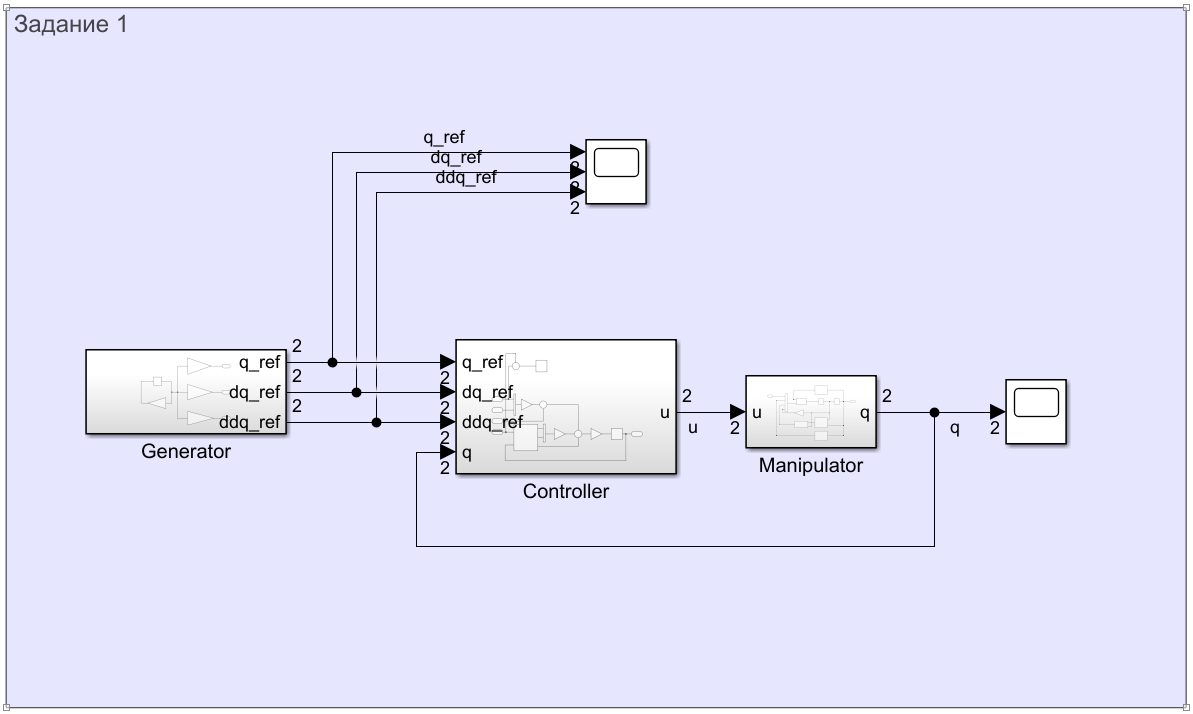
\includegraphics[width=0.75\textwidth]{global sys.png}
        \caption{Общий вид модели в MATLAB}
        \label{pic:global sys}
    \end{figure}

    Инициализация всех параметров производится с помощью автоматически вызываемой встроенной функции \texttt{InitFcn},
    где перечисленны необходимые переменные (см.~\ref{code:given}).
    \begin{figure}[H]
        \centering
        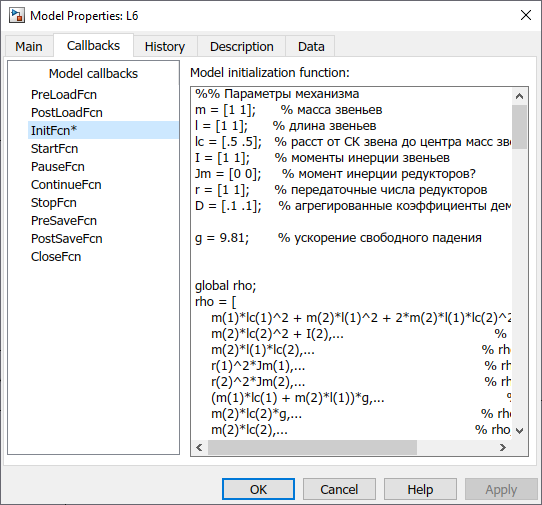
\includegraphics[height=0.3\textheight]{InitFcn.png}
        \caption{Окно \texttt{InitFcn}}
        \label{pic:InitFcn}
    \end{figure}

    \sloppy Модель манипулятора представлена на рисунке~\ref{pic:manipulator}.
    \begin{figure}[H]
        \centering
        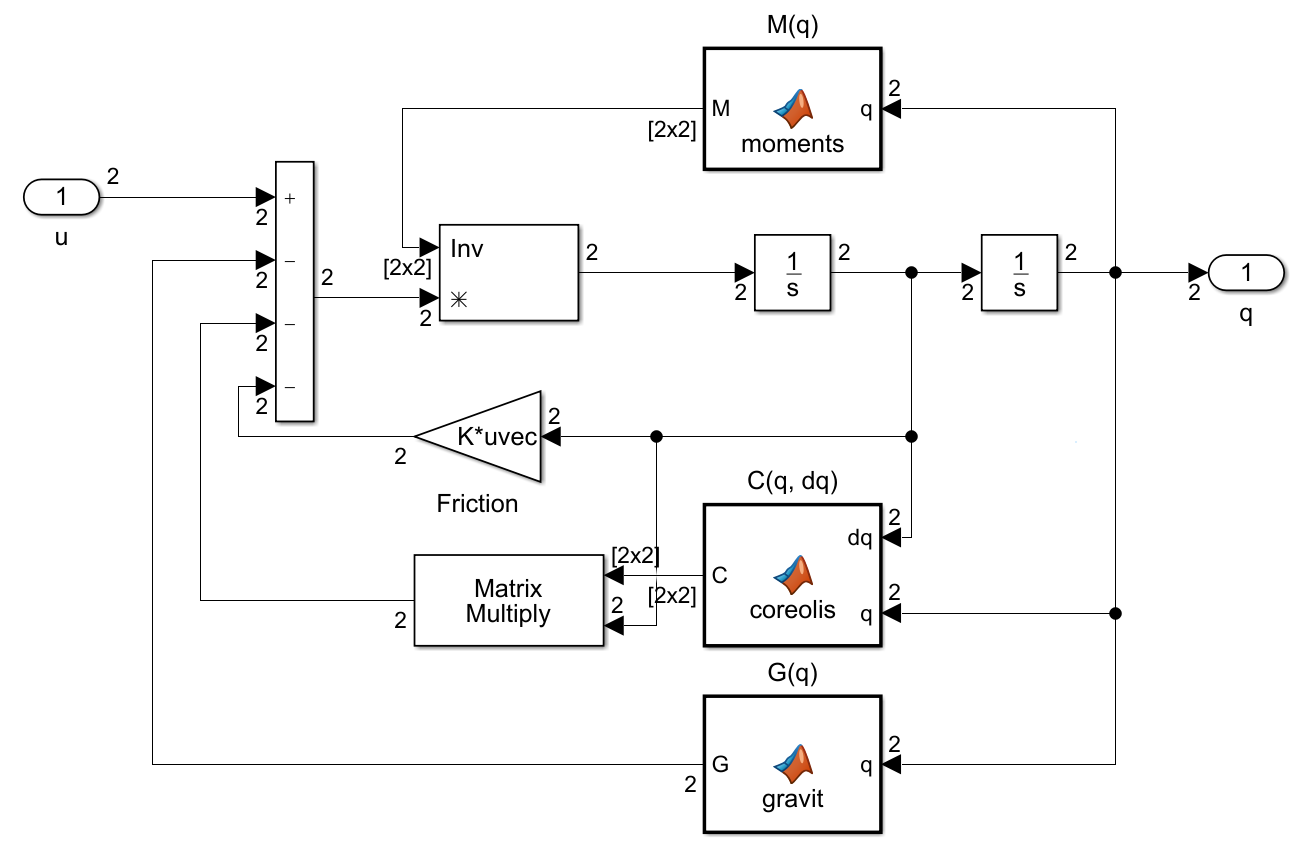
\includegraphics[width=0.75\textwidth]{manipulator.png}
        \caption{Модель манипулятора}
        \label{pic:manipulator}
    \end{figure}

    Модель регулятора представлена на рисунке~\ref{pic:controller}, а расширенный наблюдатель на
    рисунке~\ref{pic:extended observer}.
    \begin{figure}[H]
        \centering
        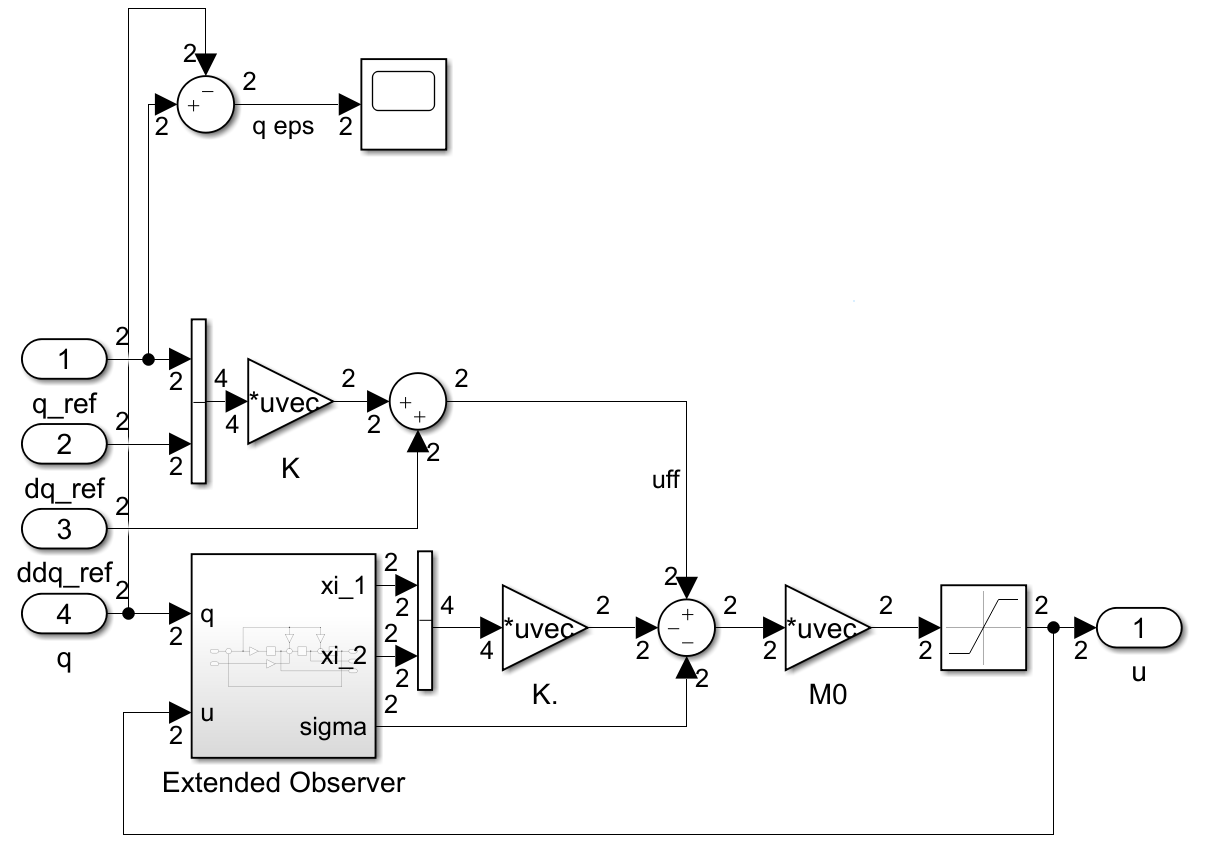
\includegraphics[width=0.75\textwidth]{controller.png}
        \caption{Модель регулятора}
        \label{pic:controller}
    \end{figure}

    \begin{figure}[H]
        \centering
        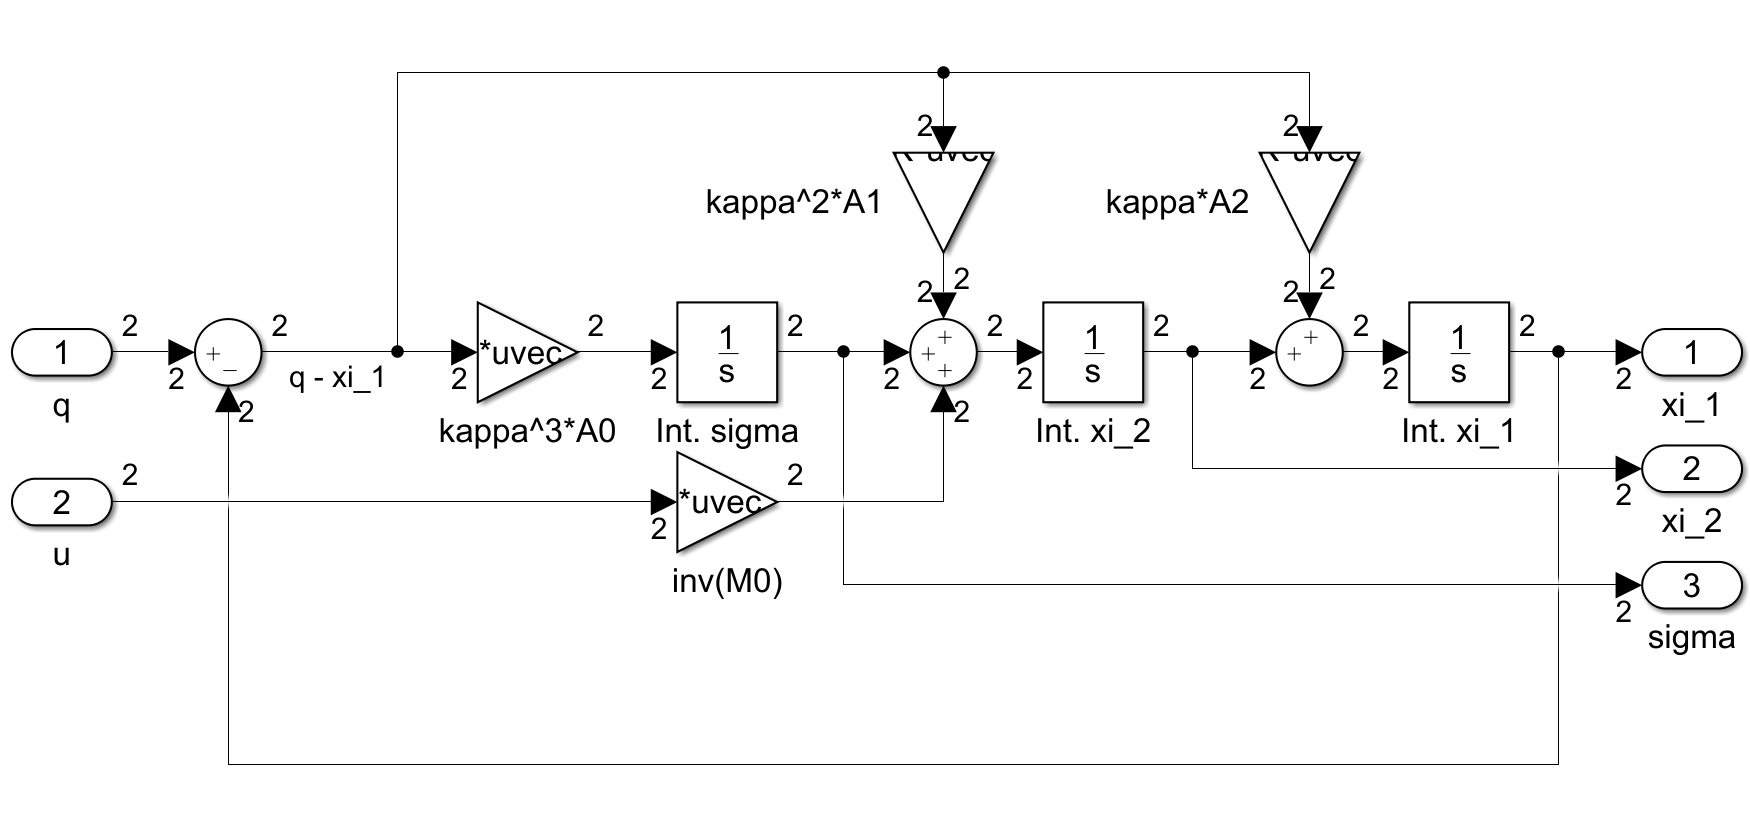
\includegraphics[width=0.75\textwidth]{extended observer.png}
        \caption{Расширенный наблюдатель}
        \label{pic:extended observer}
    \end{figure}

    Генератор задающего воздействия~\eqref{eq:traject} представлен на рисунке~\ref{pic:generator}
    \begin{figure}[H]
        \centering
        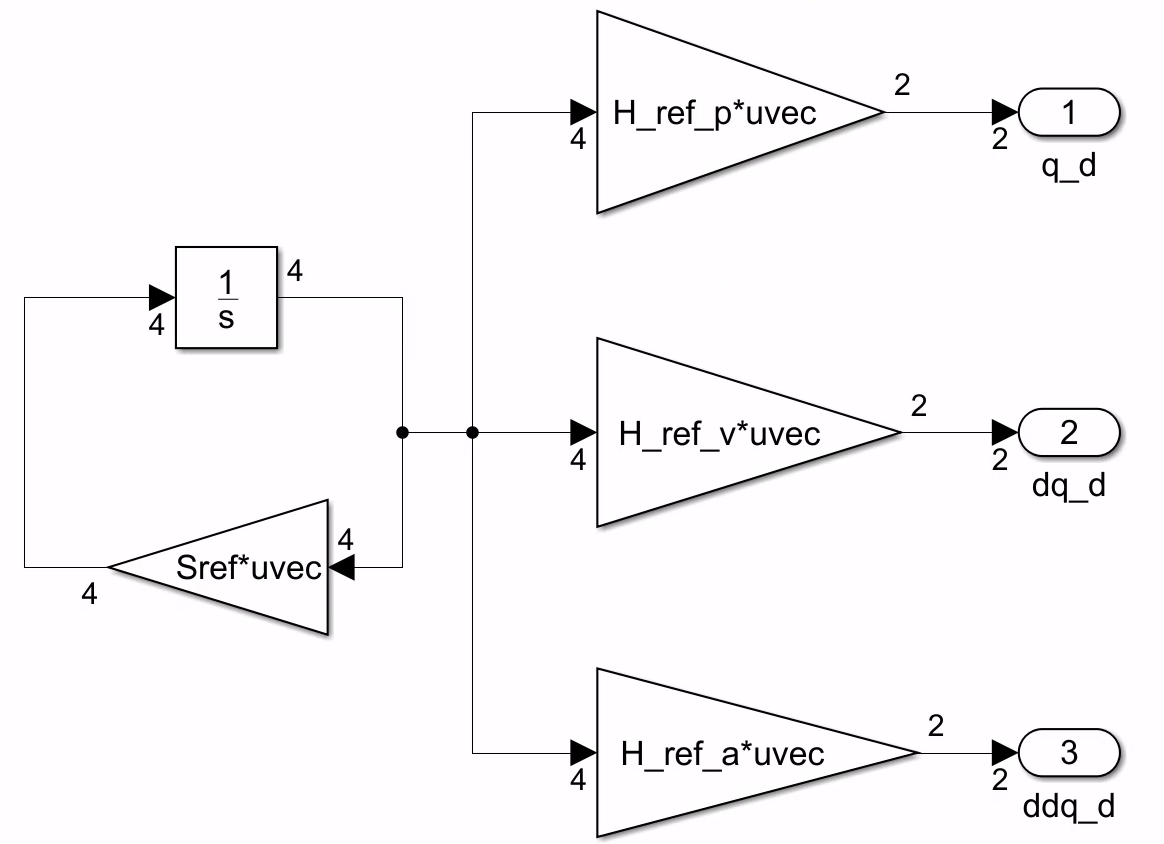
\includegraphics[width=0.75\textwidth]{generator.png}
        \caption{Модель задающего воздействия}
        \label{pic:generator}
    \end{figure}

    Результат моделирования представлен на рисунке~\ref{pic:result}. По графику очевидно, что ошибка
    положения звеньев сходится к нулю и соответственно цель моделирования~\eqref{eq:goal} выполнена.
    \begin{figure}[H]
        \centering
        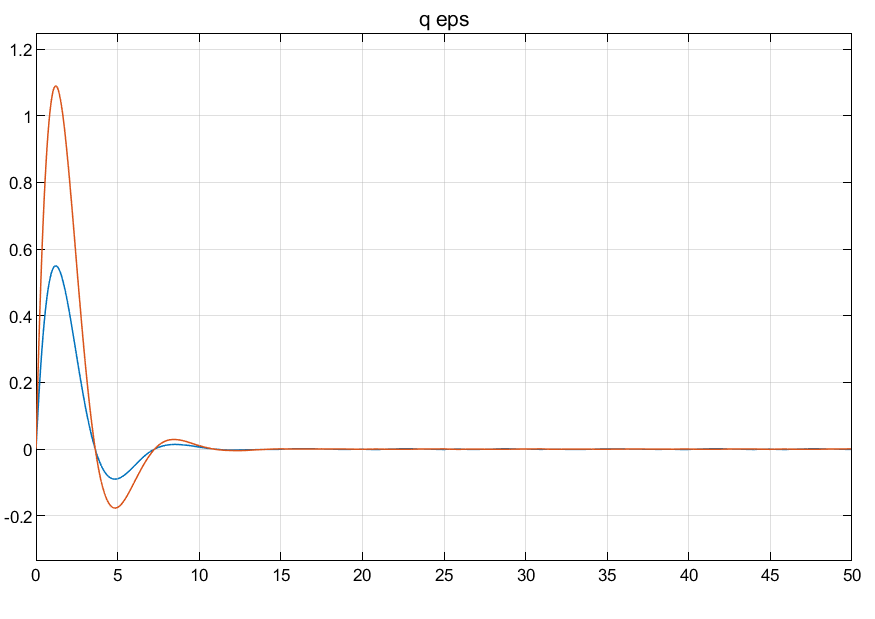
\includegraphics[width=0.75\textwidth]{result.png}
        \caption{Ошибка положения системы}
        \label{pic:result}
    \end{figure}

    \subsection*{Задание 2}
    Ослабив допущение 1 мы имеем внешнее воздействие на систему и необходимо добавить внутреннюю
    модель.

    Новая модель системы с внешним возмущением и внутренней моделью представлена на рисунке~\ref{pic:sys dist}.
    \begin{figure}[H]
        \centering
        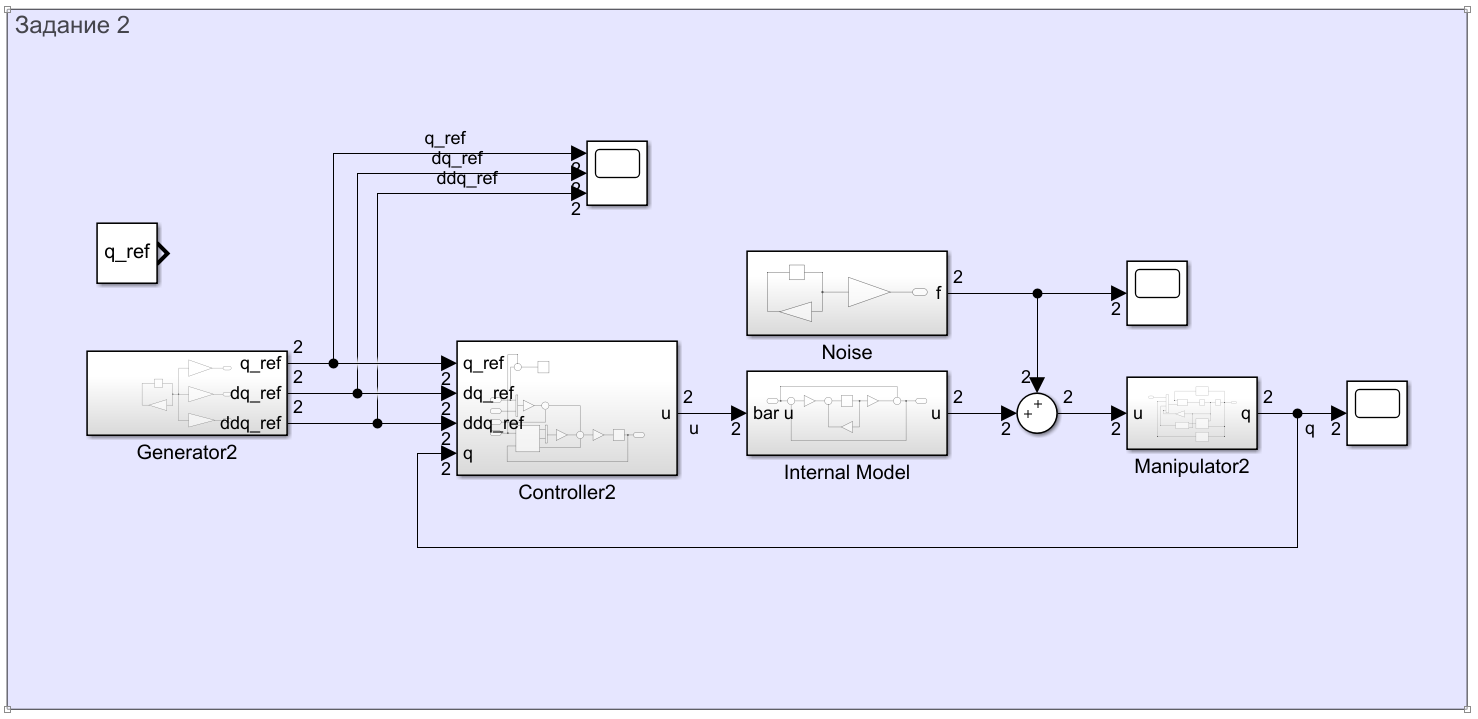
\includegraphics[width=0.75\textwidth]{sys dist.png}
        \caption{Общий вид модели}
        \label{pic:sys dist}
    \end{figure}

    Устройство внутренней модели представлено на рисунке~\ref{pic:internal model}.
    \begin{figure}[H]
        \centering
        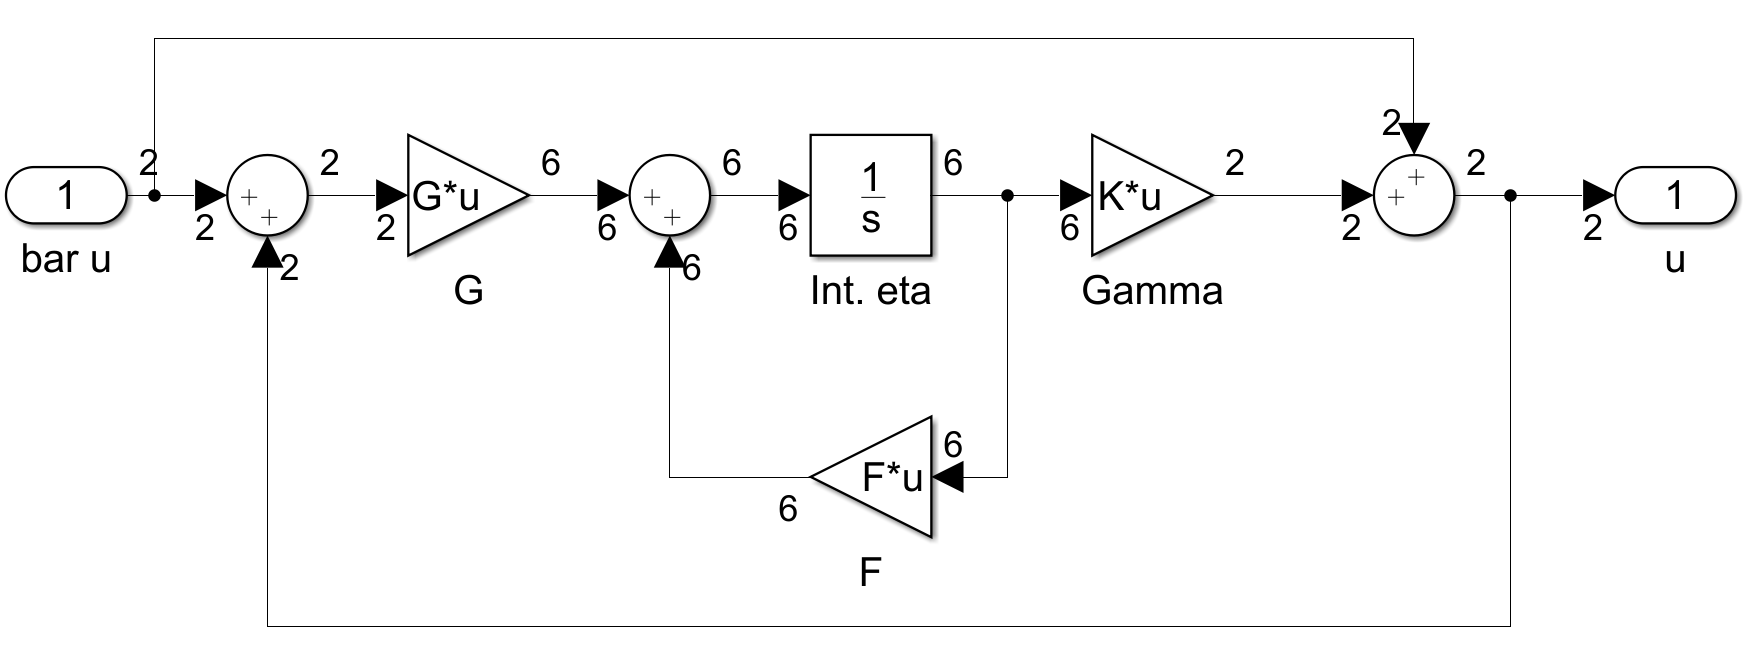
\includegraphics[width=0.75\textheight]{internal model.png}
        \caption{Внутренняя модель}
        \label{pic:internal model}
    \end{figure}

    Генератор внешнего возмущения представлен на рисунке~\ref{pic:dist generator}
    \begin{figure}[H]
        \centering
        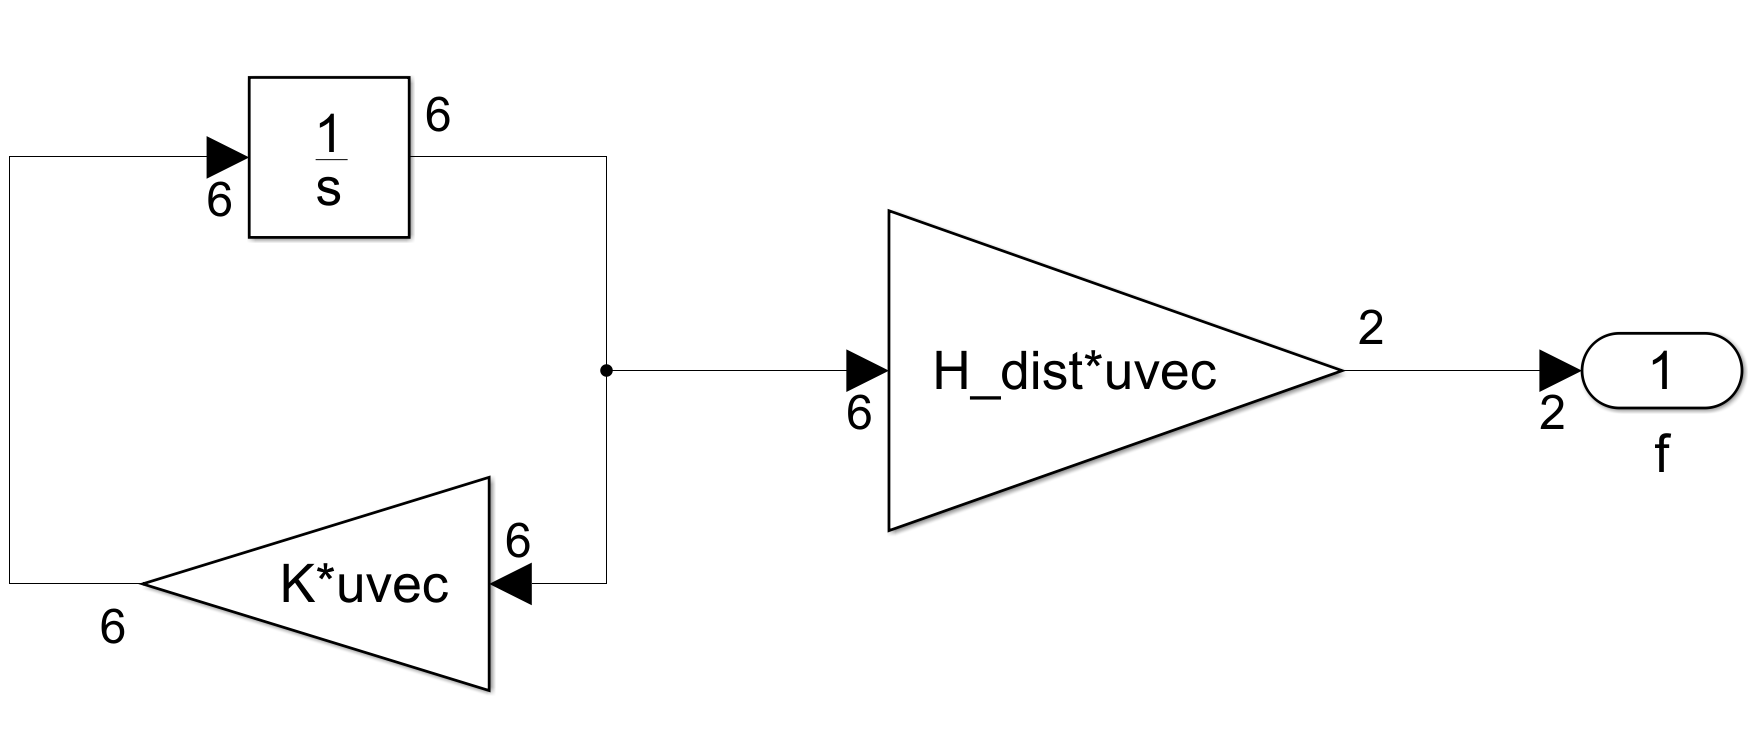
\includegraphics[width=0.75\textwidth]{dist generator.png}
        \caption{Генератор внешнего возмущения}
        \label{pic:dist generator}
    \end{figure}

    Результат моделирования представлен на рисунке~\ref{pic:result dist}. По графику очевидно, что ошибка
    положения звеньев сходится в нулю и соответственно цель моделирования~\eqref{eq:goal} выполнена.
    \begin{figure}[H]
        \centering
        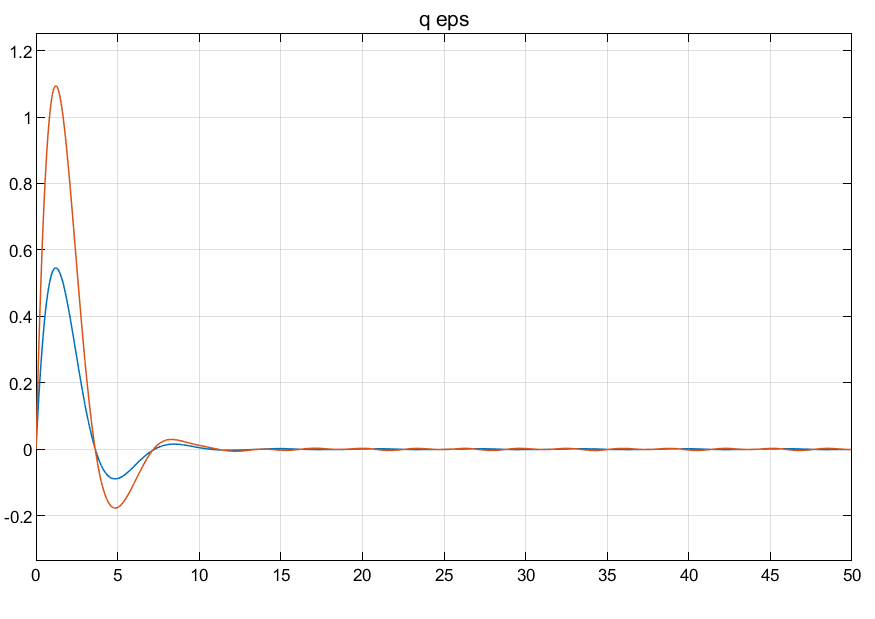
\includegraphics[width=0.75\textwidth]{result dist.png}
        \caption{Ошибка положения системы}
        \label{pic:result dist}
    \end{figure}

    \section*{Вывод}
    В работе была промоделирована система управления двухзвенным манипулятором с робастным регулятором.

    Результаты моделирования показывают, что использование дополнительной внутренней модели в системе
    на которую оказывается внешнее детерминированное воздействие позволяет успешно управлять объектом
    и ошибка положения сходится к нулю так же как и в ситуации без внешнего воздействия.

    \appendix \newpage
    \renewcommand{\thesection}{Приложение \Asbuk{section}}
    \section{Параметры инициализации}\label{code:given}
    \octavefile[frame=single]{../src/given.m}

\end{document}
